% Chris's Entropy Library - User Guide - Top Level
% Written by Christopher Thomas.

\documentclass[letterpaper,11pt]{report}
\usepackage[letterpaper]{geometry}
\usepackage{graphicx}
\usepackage{verbatim}
\usepackage{placeins}
\usepackage{longtable}
% Needed for "mathbb" (outline bold).
%\usepackage{amsfonts}

\geometry{nohead,footskip=0.3in,margin=0.75in}

% Force my paragraph style, darnit.
\usepackage{indentfirst}
\setlength{\parskip}{\baselineskip}

% NOTE - "\thispagestyle" is used for part and chapter beginning pages, and
% overrides \pagestyle. Redefine it to be harmless.
% NOTE - The canonical solution ("\pagenumbering{gobble}") resets the page
% counter whenever it's used.
\renewcommand{\thispagestyle}[1]{}

% Custom macros.
\newcommand{\fixme}[1]{\textbf{FIXME: #1}}

\newcommand{\figdef}[3]
{\begin{figure}[htb]
\begin{center}#1\end{center}
\caption{#2}\label{#3}\end{figure}}

% NOTE - This was [hb].
\newcommand{\tabdef}[3]
{\begin{table}[htb]
\begin{center}#1\end{center}
\caption{#2}\label{#3}\end{table}}

% Document body.
\begin{document}
%
% Title page.
%
\pagestyle{empty}

\begin{center}
%
\vspace*{1in}
{\Huge Chris's Entropy Library - User Guide} \\
{\footnotesize Written by Christopher Thomas -- \today.}
%
\vspace*{1.5in}\\
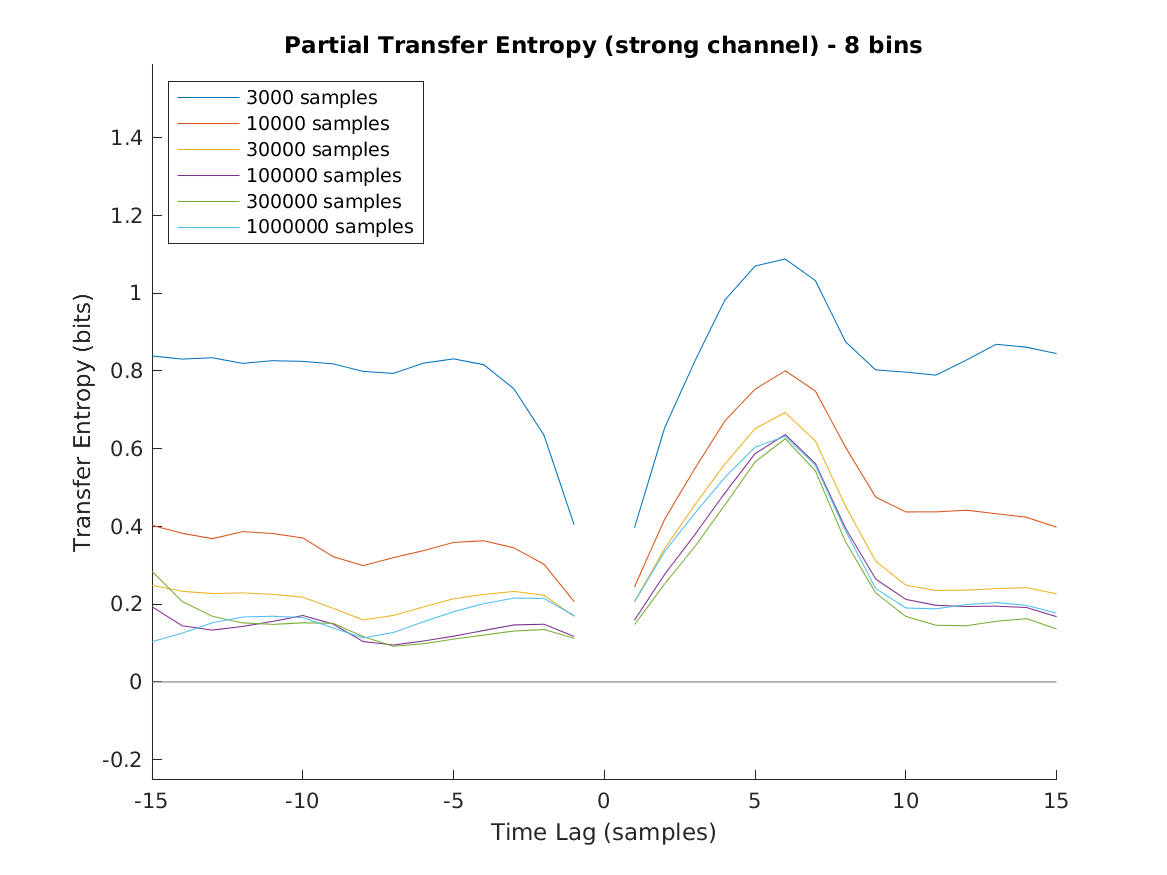
\includegraphics[width=5in]{plots/pte-strong-laglength-08bins.png}
%
\end{center}
%
\vfill
{\tiny \input{../LICENSE.md}}
%
\clearpage
%
%
% Front matter.
%
\pagestyle{plain}
\pagenumbering{roman}
\setcounter{page}{1}
%
\tableofcontents
%
\clearpage
%
%
% Document parts.
%
\pagestyle{plain}
\setcounter{page}{1}
\pagenumbering{arabic}
%
% Chris's Entropy Library - User Guide - Overview
% Written by Christopher Thomas.

\chapter{Overview}
\label{sect-over}

This library provides a set of functions used for calculating entropy and
entropy-related measures on datasets. These were written to deal with
neuroscience data (continuous brain wave signals and discrete counts of
the numbers spike events seen), but the library should work with any type
of data.

Measures computed are:

\begin{itemize}
%
\item \textbf{Shannon Entropy} - The amount of ``surprise'' associated
with a given data sample, and the average ``surprise'' for samples in a
data stream. This is the information content of the stream.
%
\item \textbf{Conditional Entropy} - The amount learned from samples of
variable Y when we already know the value of a related variable X.
%
\item \textbf{Mutual Information} - The amount of information shared by
samples of related variables Y and X. Measuring either one gets you this
information.
%
\item \textbf{Transfer Entropy} - The amount of information about the
future of variable Y that you learn by knowing the past of variable X, in
addition to what you already know from the past of variable Y.
%
\end{itemize}

These measures are discussed in detail in Section \ref{sect-entropy}.

A brief description of how to use this library is given in Section
\ref{sect-howto}. For more information, see the sample code in the
``\verb|source-code|'' folder. This section also provides a brief overview
of considerations relating to neuroscience data analysis.

Section \ref{sect-extrap} describes the quadratic extrapolation algorithm
that was used in Palmigiano 2017. This is intended to allow reliable
estimates of several entropy measures with fewer data samples than would
otherwise be needed (or equivalently, to improve the reliability of these
measures using a fixed number of samples).

%
% This is the end of the file.

% Chris's Entropy Library - User Guide - Entropy
% Written by Christopher Thomas.

\chapter{Entropy}
\label{sect-entropy}

\section{Shannon Entropy}
\label{sect-entropy-shannon}

\textbf{Entropy} can be thought of as measuring the information content of
a stream of data samples. It is defined (per Shannon 1949) as the amount of
``surprise'' associated with each sample when that sample is considered to
be a discrete symbol drawn from a set of possible symbols with some
probability distribution. The entropy associated with one symbol is given
in Equation \ref{eq-shannon-symbol}, and the average entropy per symbol
associated with a symbol stream is given in Equation
\ref{eq-shannon-stream}. It can be seen from Equation \ref{eq-shannon-symbol}
that symbols with lower probability result in more ``surprise'': rare symbols
are more informative than commonly-seen symbols.

\begin{equation}
H(x_k) = \log_2 \left [ \frac{1}{P(x_k)} \right ] = - \log_2 [ P(x_k) ]
\label{eq-shannon-symbol}
\end{equation}

\begin{equation}
H(X) = - \sum_k P(x_k) \log_2 [ P(x_k) ]
\label{eq-shannon-stream}
\end{equation}

For discrete-valued data, or data such as text that is readily interpreted
as symbols, entropy may be calculated on the raw data values. A histogram
of observed symbols is made, and this is used as the probability
distribution. For continuous-valued data, histogram bins are typically
defined and the bin labels are interpreted as symbols. For data consisting
of event arrival times, time bins are typically defined and the number of
events within each bin are counted. These counts may be taken as individual
symbols or several adjacent time bins may be considered to form a word,
which is used as a symbol for entropy calculations. These approaches are
discussed in more detail in Section \ref{sect-howto}.

% FIXME - Force a page break.
\clearpage
%
\section{Conditional Entropy}
\label{sect-entropy-cond}

\textbf{Conditional entropy} can be thought of as the amount of additional
information learned from samples of variable Y when we already know the
value of a related variable X. This is illustrated in Figure
\ref{fig-cond-def}. It is defined by Equation \ref{eq-cond-def}:

\begin{equation}
H(Y|X) = - \sum_{j,k} P(x_j,y_k) \log_2 \left [
\frac{P(x_j,y_k)}{P(x_j)} \right ]
\label{eq-cond-def}
\end{equation}

For the case of independent variables where $P(x_j,y_k) = P(x_j) P(y_k)$,
this reduces to Shannon entropy.

\fixme{Figure for conditional entropy.}

This is generalized to several X variables per Equation \ref{eq-cond-multi};
this case is illustrated in Figure \ref{fig-cond-multi}.

\begin{equation}
H(Y|X_A,X_B) = - \sum_{j,k,m} P(x_{aj},x_{bk},y_m) \log_2 \left [
\frac{P(x_{aj},x_{bk},y_m)}{P(x_{aj},x_{bk})} \right ]
\label{eq-cond-multi}
\end{equation}

\fixme{Figure for conditional entropy with multiple X.}

% FIXME - Force a page break.
\clearpage
%
\section{Mutual Information}
\label{sect-entropy-mutual}

\textbf{Mutual information} can be thought of as the amount of information
shared between related variables X and Y. Sampling either variable X
\textit{or} variable Y reveals the shared information. This is illustrated
in Figure \ref{fig-mutual-def}. Mutual information is defined by
Equation \ref{eq-mutual-def}:

\begin{equation}
I(X,Y) = \sum_{j,k} P(x_j,y_k) \log_2 \left [
\frac{P(x_j,y_k)}{P(x_j) P(y_k)} \right ]
\label{eq-mutual-def}
\end{equation}

For the case of independent variables where $P(x_j,y_k) = P(x_j) P(y_k)$,
this is equal to zero (due to the $log_2(1)$ term).

\fixme{Figure for mutual information.}

This is generalized to more than two variables per Equation
\ref{eq-mutual-multi}; this case is illustrated in Figure
\ref{fig-mutual-multi}.

\begin{equation}
I(X,Y,Z) = \sum_{j,k,m} P(x_j,y_k,z_m) \log_2 \left [
\frac{P(x_j,y_k,z_m)}{P(x_j) P(y_k) P(z_m)} \right ]
\label{eq-mutual-multi}
\end{equation}

\fixme{Figure for mutual information with three variables.}

% FIXME - Force a page break.
\clearpage
%
\section{Transfer Entropy}
\label{sect-entropy-transfer}

\textbf{Transfer entropy} can be thought of as the amount of information
about the future of variable Y that you learn by knowing the past of
variable X, in addition to what you already know from the past of variable
Y. This is illustrated in Figure \ref{fig-transfer-def}. Transfer entropy
is defined by Equation \ref{eq-transfer-def}:

\begin{equation}
TE_{X \rightarrow Y} = H(Y|Y_{past}) - H(Y|Y_{past},X_{past})
\label{eq-transfer-def}
\end{equation}

The $Y_{past}$ and $X_{past}$ terms are usually approximated by taking the
past value at some time $t-\delta t$ as a proxy for the entire past history:

\begin{equation}
\begin{array}{cc}
\hat{Y}_{past} = Y(t - \delta t) \\
\hat{X}_{past} = X(t - \delta t) \\
\end{array}
\label{eq-transfer-past}
\end{equation}

\fixme{Figure for transfer entropy.}

\textbf{Partial transfer entropy} is used to disentangle the contributions
of multiple X variables to some Y variable. This is illustrated in Figure
\ref{eq-transfer-pte}. Partial transfer entropy is defined by Equation
\ref{eq-transfer-pte}:

\begin{equation}
pTE_{X_A \rightarrow Y} = H(Y_A|Y_{past},X_{Bpast})
- H(Y|Y_{past},X_{Apast},X_{Bpast})
\label{eq-transfer-pte}
\end{equation}

\fixme{Figure for partial transfer entropy.}

\section{References}
\label{sect-entropy-refs}

\begin{itemize}
%
\item C. E. Shannon, \textit{A Mathematical Theory of Communication},
The Bell System Technical Journal, v~27, pp~379--423,623-656, July, October,
1948
%
\end{itemize}

%
% This is the end of the file.

%% Chris's Entropy Library - User Guide - How-To Guide
% Written by Christopher Thomas.

\chapter{Using This Library}
\label{sect-howto}

\iffalse
A brief description of how to use this library is given in Section
\ref{sect-howto}. For more information, see the sample code in the
``\verb|source-code|'' folder. This section also provides a brief overview
of considerations relating to neuroscience data analysis.
\fi

%
% This is the end of the file.

%% Conditional Entropy Library - User Guide - Quadratic Extrapolation
% Written by Christopher Thomas.

\chapter{Quadratic Extrapolation}
\label{sect-extrap}

This library's calculations of conditional entropy, mutual information,
and transfer entropy are estimates. These estimates converge on the true
values as the number of samples is increased. A rigorous analysis of the
effect of small sample sizes on estimates typically performed with neural
data is presented in Treves 1995. The take-away from that work is that
entropy tends to be over-estimated, and that the estimate tends to converge
monotonically on the correct value as sample size is increased. An example
of this convergence for mutual information estimated using this library is
shown in Figure \ref{fig-extrap-mi} (left pane).

A follow-up analysis presented in Strong 1998 showed that for sample counts
above a threshold, the true entropy value could be estimated by
curve-fitting estimates from finite sample counts and extrapolating the
curve fit to infinite sample counts. An example of applying this
extrapolation method to mutual information estimation using this library is
shown in Figure \ref{fig-extrap-mi} (right pane). Note that the estimate
converges more quickly but is no longer monotonic.

\figdef{\begin{tabular}{ccc}
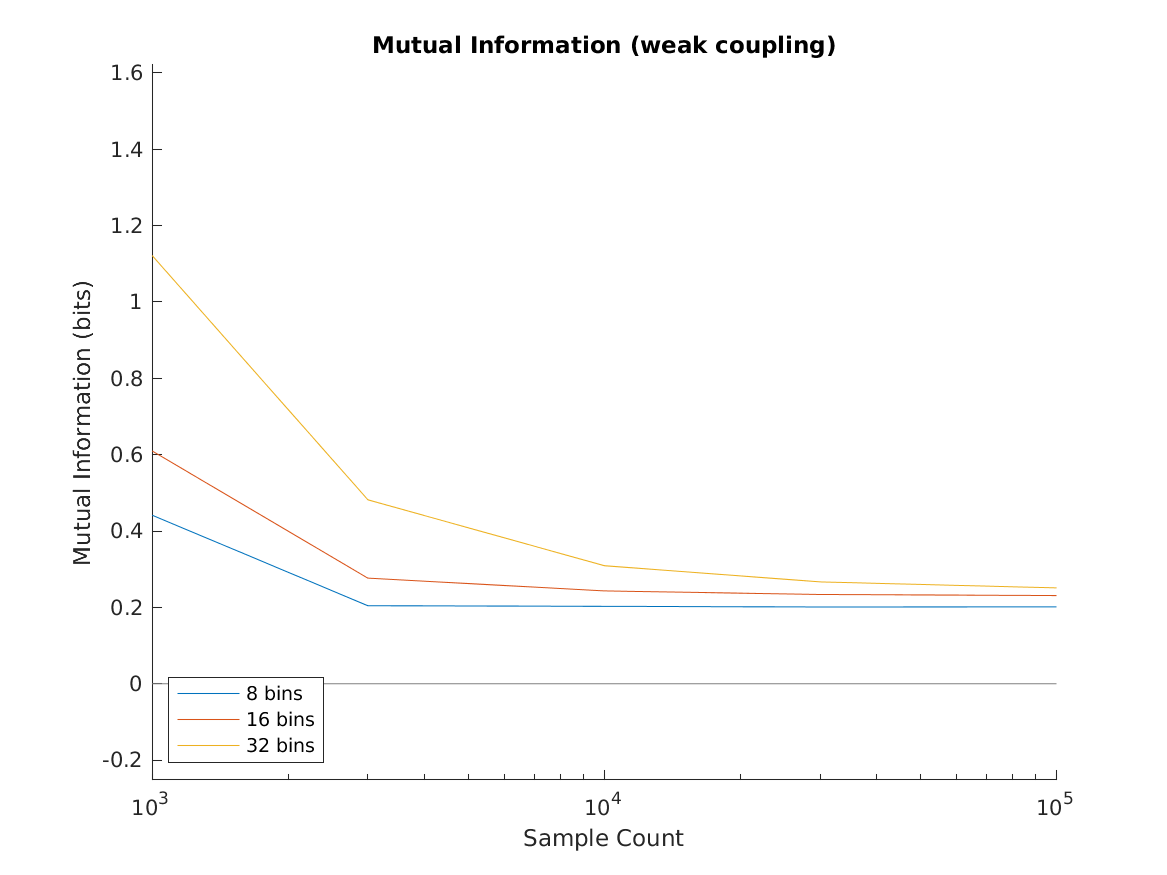
\includegraphics[width=0.45\textwidth]{plots/mutual-weak-raw.png} & ~ &
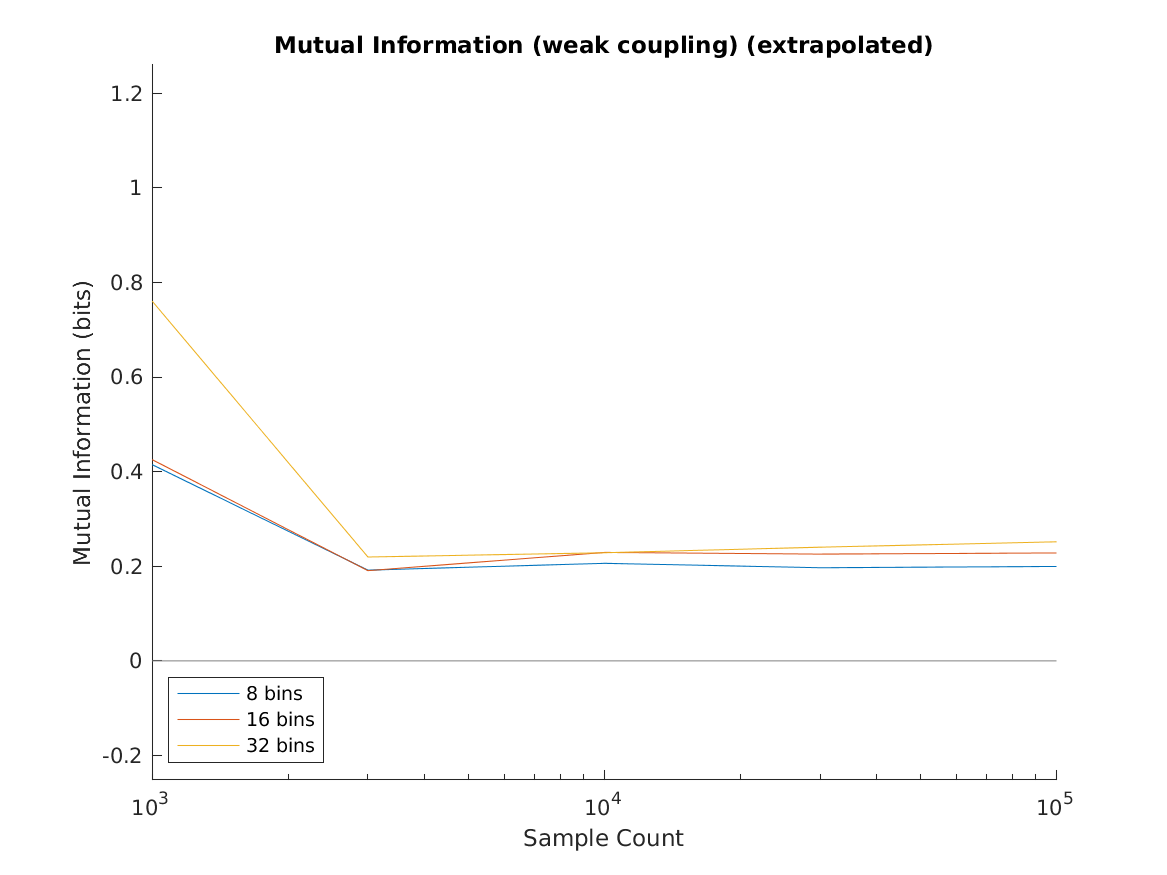
\includegraphics[width=0.45\textwidth]{plots/mutual-weak-extrap} \\
\end{tabular}}
{Mutual information between weakly coupled signals computed without
extrapolation (left) and with extrapolation (right), as a function of the
number of samples used to produce the estimate.}
{fig-extrap-mi}

This library's implementation of the extrapolation algorithm is based on
description given in Palmigiano 2017, used in that work for the estimation
of transfer entropy. In this library it may be used (at the user's
discretion) for the estimation of conditional entropy, mutual information,
and transfer entropy.

The algorithm is supplied with several divisor values $N_{div}$. For each
divisor value several random subsets of the data of size $N_{samp}
\div N_{div}$ are chosen. The metric to be estimated is evaluated for each
of these random subsets, and the results are averaged to produce an estimate
associated with that $N_{div}$. A quadratic curve fit is performed as a
function of $N_{div}$. This is used to estimate the metric value at
$N_{div} = 0$, which corresponds to an infinite number of samples.

As noted in Strong 1998, there is a minimum sample count below which this
estimation method fails. With or without quadratic extrapolation, it will
be necessary to test several sample counts to evaluate whether the estimate
has converged or not. In testing, the practical impact of extrapolation was
to reduce the number of samples needed for convergence by approximately
$3\times$ to $10\times$.

\section{References}
\label{sect-extrap-refs}

\begin{itemize}
%
\item A. Treves, S. Panzeri, \textit{The Upward Bias in Measures of
Information Derived from Limited Data Samples}, Neural computation,
v~7, pp~399-407, 1995
%
\item S. P. Strong, R. Koberle, R. R. de Ruyter van Steveninck, W. Bialek,
\textit{Entropy and Information in Neural Spike Trains},
Physical Review Letters, v~80, no.~1, pp~197-200, January 1998
%
\item A. Palmigiano, T. Geisel, F. Wolf, D. Battaglia,
\textit{Flexible Information Routing by Transient Synchrony},
Nature Neuroscience, v~20, no.~7, pp~1014-1022, 2017
%
\end{itemize}

%
% This is the end of the file.

%
%
\end{document}

%
% This is the end of the file.
